\section{Experiments}
\label{sec:experiments}

We evaluate KFAC-Muon on image classification tasks where Muon is already a strong baseline. Our goal in these experiments is not yet to provide a fully exhaustive benchmark suite, but to test whether applying Muon in KFAC-whitened coordinates improves optimization over standard Muon under comparable training recipes. Unless otherwise stated, the results below are single-seed runs and should be interpreted as preliminary.

\subsection{Setup}
\label{sec:experiments-setup}

\paragraph{Datasets and models.}
We consider two vision-transformer settings. First, we train a ViT-S/16 model on CIFAR-100. CIFAR-100 is converted to an ImageFolder-style dataset and trained using the standard ViT image pipeline. Second, we train a ViT-B/16 model on ImageNet-100, a 100-class subset of ImageNet. The ImageNet-100 runs use the same model, data processing, batch size, learning-rate schedule, augmentation, and regularization for Muon and KFAC-Muon.

\paragraph{Training recipe.}
For ImageNet-100, we train ViT-B/16 for 90 epochs with batch size 256, cosine learning-rate decay, 5 warmup epochs, base learning rate $10^{-3}$, minimum learning rate $10^{-5}$, weight decay 0.07, Mixup 0.2, CutMix 0.2, label smoothing 0.1, stochastic depth 0.1, random erasing probability 0.1, and bfloat16 AMP. KFAC-Muon uses damping $5 \times 10^{-5}$, Muon scale parameter $\epsilon=0.012$, KFAC momentum 0.9, KFAC factor/statistics updates every 2 optimizer steps, KFAC factor EMA 0.95, inverse factors computed in bfloat16, and static damping. For the ImageNet-100 ViT-B/16 runs, KFAC-Muon is applied to all affine layers, including the patch embedding and classifier head.

For CIFAR-100, we train ViT-S/16 for 75 epochs with batch size 128, cosine learning-rate decay, weight decay 0.07, Mixup 0.2, CutMix 0.2, label smoothing 0.1, stochastic depth 0.1, random erasing probability 0.1, and bfloat16 AMP. We compare against tuned Muon baselines with learning rates $10^{-3}$ and $1.2\times 10^{-3}$. The main KFAC-Muon CIFAR-100 run uses learning rate $5.5\times 10^{-4}$ with RMS matching, static damping $5\times 10^{-5}$, Muon scale parameter $\epsilon=0.038$, KFAC momentum 0.9, factor/statistics updates every 2 optimizer steps, and factor EMA 0.95. As in the ImageNet-100 run, KFAC-Muon is applied to the first and last affine layers.

\subsection{Main results}
\label{sec:experiments-main-results}

Table~\ref{tab:main-results} reports best and final validation performance. KFAC-Muon improves over the best Muon baseline in both settings. On CIFAR-100 with ViT-S/16, KFAC-Muon improves best top-1 accuracy by 2.17 points and reduces validation loss from 1.167 to 1.084. On ImageNet-100 with ViT-B/16, under a matched 90-epoch batch-256 recipe, KFAC-Muon improves final top-1 accuracy by 1.76 points and reduces validation loss from 0.854 to 0.807.

\begin{table}[t]
\centering
\caption{Main single-seed validation results. Best and final top-1 are equal for these runs because the best checkpoint occurs at the final epoch.}
\label{tab:main-results}
\begin{tabular}{llrrrr}
\toprule
Dataset / model & Optimizer & Epochs & Best top-1 & Final top-1 & Final loss \\
\midrule
CIFAR-100 / ViT-S/16 & Muon & 75 & 73.53 & 73.53 & 1.167 \\
CIFAR-100 / ViT-S/16 & KFAC-Muon & 75 & 75.70 & 75.70 & 1.084 \\
ImageNet-100 / ViT-B/16 & Muon & 90 & 82.30 & 82.30 & 0.854 \\
ImageNet-100 / ViT-B/16 & KFAC-Muon & 90 & 84.06 & 84.06 & 0.807 \\
\bottomrule
\end{tabular}
\end{table}

Figure~\ref{fig:cifar100-curves} shows the CIFAR-100 top-1 learning curves and the pointwise top-1 gap relative to the stronger Muon baseline. The KFAC-Muon run finishes with the highest validation accuracy and the lowest validation loss in Table~\ref{tab:main-results}. We also ran a longer 200-epoch CIFAR-100 sanity check, where KFAC-Muon reached 75.86\% best top-1 compared with 74.83\% for Muon, supporting the same direction of effect.

\begin{figure}[t]
\centering
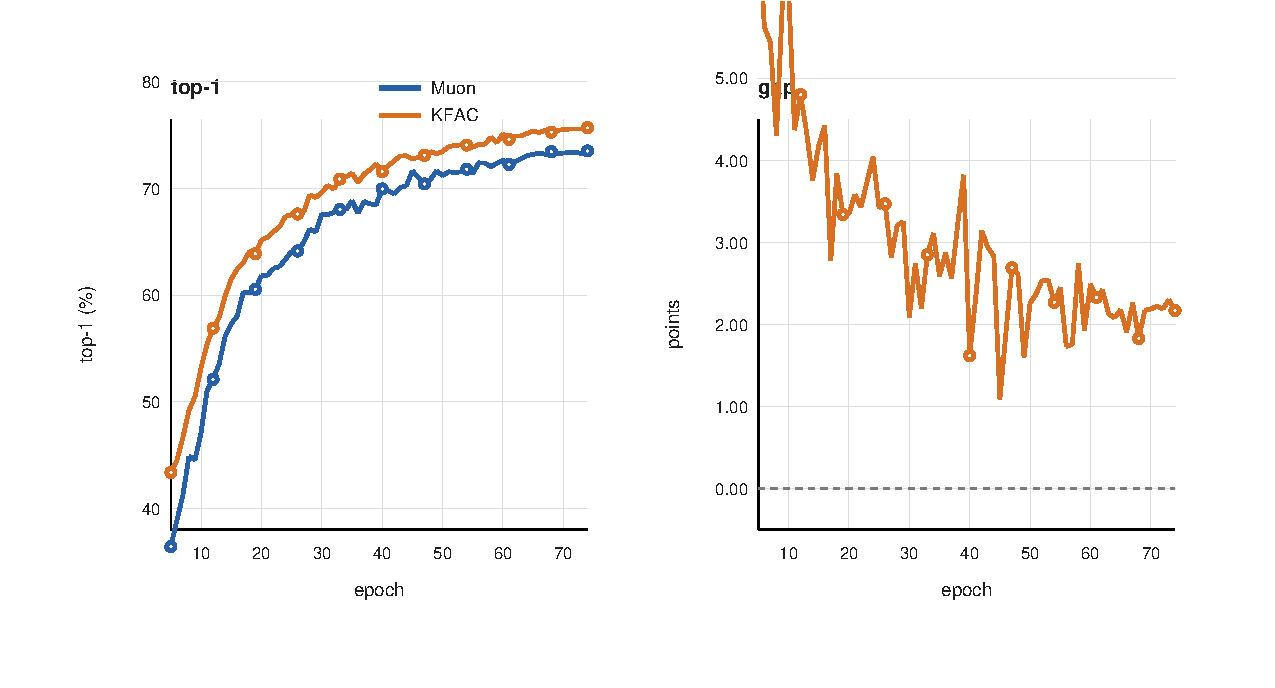
\includegraphics[width=\linewidth]{notes/figures/cifar100_vits16_curves.pdf}
\caption{CIFAR-100 ViT-S/16 validation top-1 curves and pointwise top-1 gap. The right panel plots KFAC-Muon minus Muon in percentage points.}
\label{fig:cifar100-curves}
\end{figure}

Figure~\ref{fig:imagenet100-curves} shows the matched ImageNet-100 comparison and the pointwise top-1 gap. KFAC-Muon is ahead early in training and remains ahead through the end of the run. The gap is largest during the early and middle stages of training, but remains 1.76 top-1 points at epoch 90. KFAC-Muon also reaches several accuracy thresholds earlier: for example, it reaches 82\% top-1 at epoch 64, while Muon reaches 82\% at epoch 85.

\begin{figure}[t]
\centering
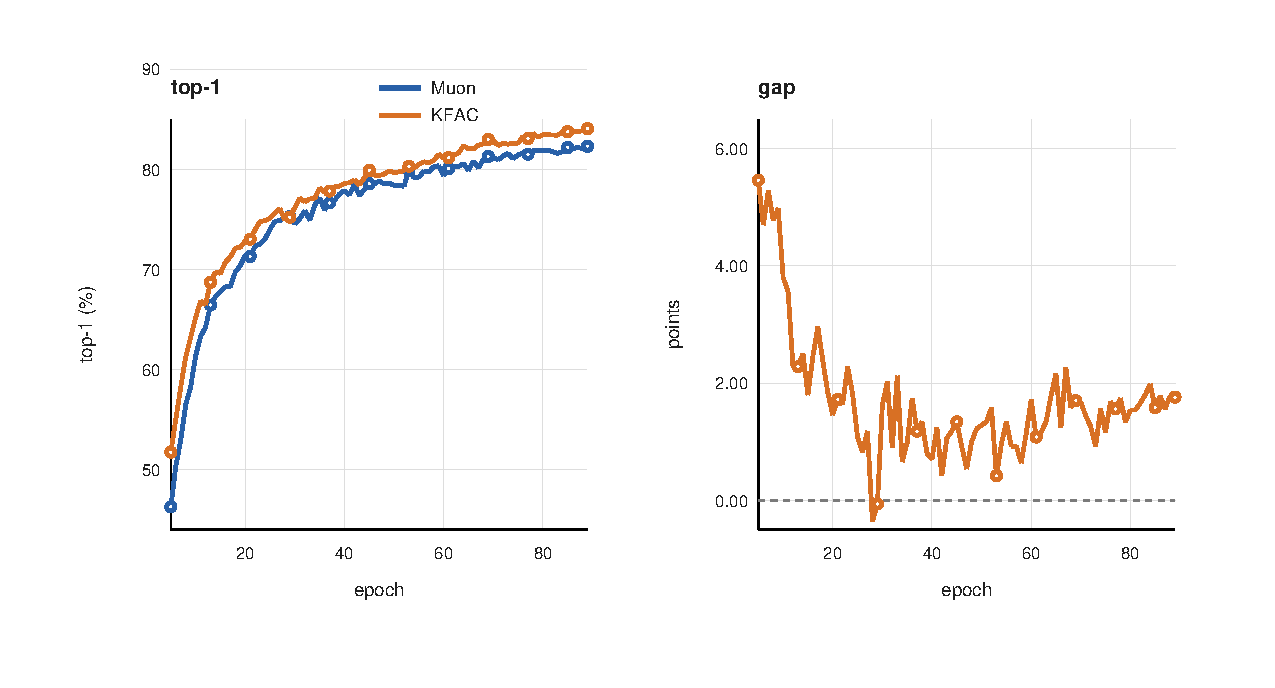
\includegraphics[width=\linewidth]{notes/figures/imagenet100_vitb16_b256_curves.pdf}
\caption{ImageNet-100 ViT-B/16 validation top-1 curves and pointwise top-1 gap with matched batch size 256 and 90-epoch schedule. The right panel plots KFAC-Muon minus Muon in percentage points.}
\label{fig:imagenet100-curves}
\end{figure}

\begin{figure}[t]
\centering
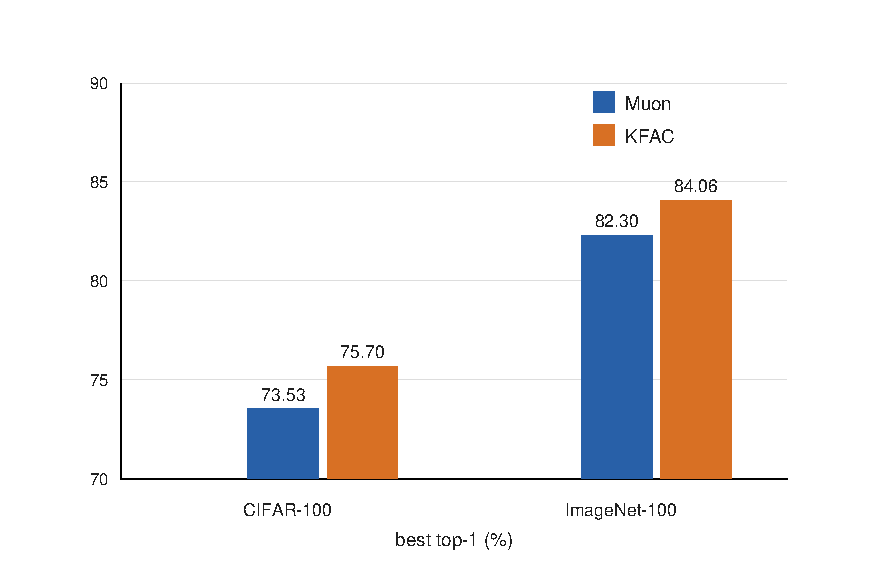
\includegraphics[width=0.82\linewidth]{notes/figures/main_results_best_top1.pdf}
\caption{Best validation top-1 accuracy for the main CIFAR-100 and ImageNet-100 runs.}
\label{fig:main-results-bars}
\end{figure}

Figure~\ref{fig:loss-curves} shows validation loss for the same main comparisons. The loss curves agree with the top-1 results: KFAC-Muon reaches lower validation loss on both CIFAR-100 and ImageNet-100.

\begin{figure}[t]
\centering
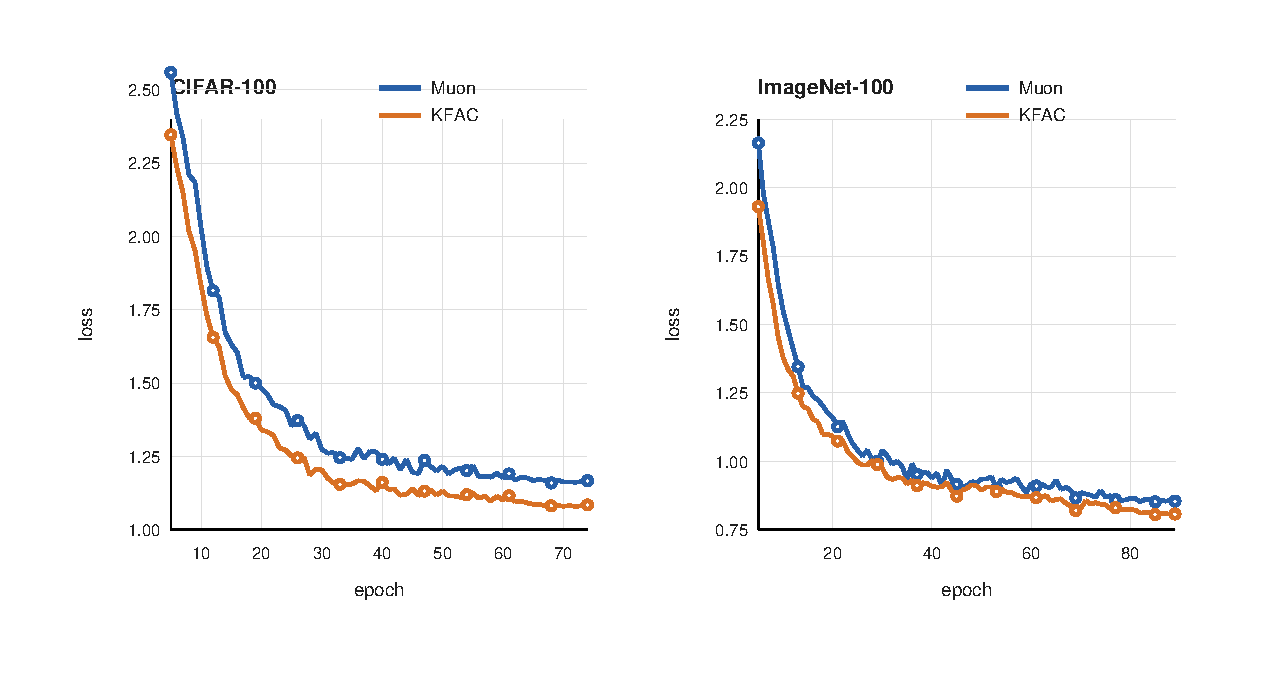
\includegraphics[width=\linewidth]{notes/figures/validation_loss_curves.pdf}
\caption{Validation loss curves for the main CIFAR-100 and ImageNet-100 comparisons.}
\label{fig:loss-curves}
\end{figure}

\subsection{Comparison to FISMO-style factor estimation}
\label{sec:experiments-fismo}

The experiments above use classical activation/output-gradient KFAC factors. A direct comparison to FISMO-style factor estimation should use the same whiten--polar--unwhiten update while replacing the KFAC activation and output-gradient covariances with the corresponding gradient-derived Kronecker factors. We have not yet completed this controlled comparison for the final ImageNet-100 recipe. This is an important next experiment because it isolates whether the improvement comes from the Fisher-whitened Muon template itself or from the specific KFAC estimator used to define the whitening geometry.

\subsection{Ablations}
\label{sec:experiments-ablations}

\paragraph{Layer coverage.}
For ViT-B/16 on ImageNet-100 and ViT-S/16 on CIFAR-100, applying KFAC-Muon to the patch embedding and classifier head was important. Earlier pilot runs that excluded the first and last affine layers were weaker, even when the KFAC step scale was increased. Including these layers made the KFAC-Muon pilot runs substantially stronger. This suggests that optimizer coverage matters for ViTs: the patch embedding is the first learned projection from pixels into token space, and the classifier head is the final map into the task-specific label space.

\paragraph{Damping and step scale.}
We swept damping and Muon scale parameters before selecting the ImageNet-100 setting in Table~\ref{tab:main-results}. Damping that was too small increased the KFAC step size but did not consistently improve validation accuracy. At batch size 256, damping $5\times 10^{-5}$ was at least as good as nearby lower damping values in 25-epoch pilots. Increasing the KFAC-Muon scale from $\epsilon=0.010$ to $\epsilon=0.012$ gave a small improvement in the 25-epoch pilot and was used for the 90-epoch run.

\paragraph{Factor update frequency.}
We found that updating KFAC statistics and factors every 2 optimizer steps was a useful compromise for the ViT runs. Less frequent updates are cheaper, but they increase factor staleness. More frequent updates increase overhead. The main ImageNet-100 run therefore uses statistics and factor updates every 2 steps.

\paragraph{Batch size.}
The ImageNet-100 result uses batch size 256. This is closer to common ViT training recipes than our earlier batch-size-64 pilots. The batch-size-256 comparison is also stricter because both Muon and KFAC-Muon use the same number of optimizer updates per epoch. Under this matched setting, KFAC-Muon reaches similar or better accuracy with the same update budget.

\subsection{Runtime and memory}
\label{sec:experiments-runtime}

KFAC-Muon introduces additional overhead from collecting activation and output-gradient statistics, forming damped factors, and applying the preconditioner before and after the Newton--Schulz orthogonalization. We use inverse factors computed in bfloat16 for the main ImageNet-100 run, which was substantially faster than earlier solve-based implementations in pilot profiling. The final runtime table is still incomplete: for a polished version of this section, we should report matched wall-clock time, peak memory, and examples/sec for the final batch-size-256 Muon and KFAC-Muon runs on the same hardware.

\subsection{Diagnostics}
\label{sec:experiments-diagnostics}

The ImageNet-100 KFAC-Muon run does not show signs of late-training instability. Although the validation accuracy is somewhat noisy from epoch to epoch, the best accuracy occurs at the final epoch, and validation loss remains below the Muon baseline throughout late training. The KFAC effective step ratio follows the learning-rate schedule: it peaks near the end of warmup and then decays smoothly with the cosine schedule. This suggests that the selected damping and step scale are not causing uncontrolled late-training updates.
